En esta sección se describe el procedimiento para obtener la curva de calibración que se usó, así como detalles técnicos del montaje experimental y los implementos que se requirieron. 
\section{Procedimiento de irradiación}
Los procedimientos de irradiación se realizaron con un acelerador True Bream de  Varian, operado a 6 $ MeV$ con filtro aplanador. Este acelerador fue calibrado con cámara de ionización siguiendo el protocolo TRS 398 para comprobar la fiabilidad de que la dosis entregada correspondiera con las unidades monitor requeridas. Una fotografía del montaje usado en el procedimiento se muestra en la figura \ref{fig:fotoMontaje}.\\

\begin{figure}
	\centering
	% \missingfigure is from todonotes
	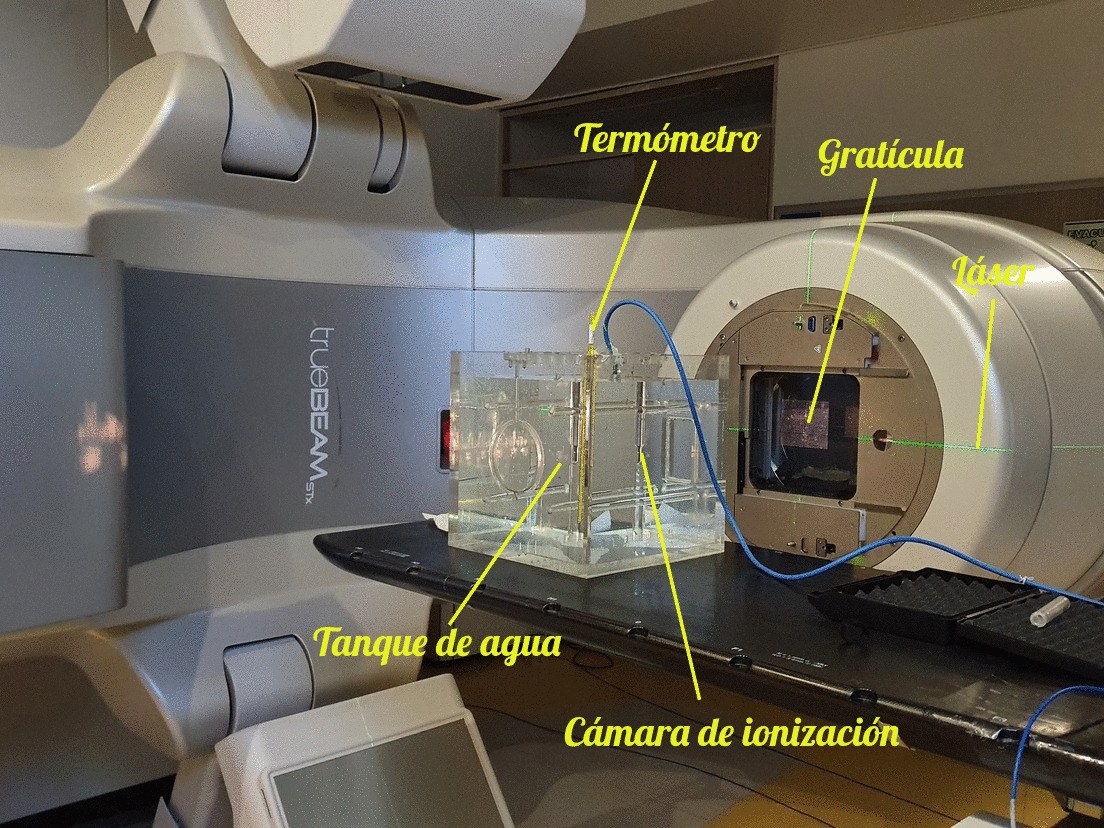
\includegraphics[width=0.7\linewidth]{images/TRS398Editado2.jpg}
	\caption{Montaje de calibración del acelerador}
	\label{fig:fotoMontaje}
\end{figure}
Para obtener la curva se irradiaron fragmentos de películas EBT3 del mismo lote de aproximadamente 5 cm x 5 cm, cortados manualmente con un bisturí. El proceso de corte despega la lamina protectora de la película, por lo que se debe tener en cuenta no usar las regiones cercanas al corte en la obtención de medidas para la calibración, puesto que cambian las propiedades ópticas con respecto a la región lejana al corte. Por otro lado, toda manipulación de las películas se realizó con guantes de nitrilo para no dejar residuos que podrían tener cierto efecto en la medida de la transmitancia. \\

Para la irradiación se alineó, con la ayuda de luz de campo, la gratícula del acelerador, los láseres del cuarto de tratamiento, y el telémetro incorporado en el acelerador, cada trozo de película con el isocentro del acelerador. Cada película fue irradiada en el centro de un campo de 20 x 20 cm a 100 cm del foco para lograr uniformidad de campo en la región donde se encuentra la película. Además, se usaron 5 cm de agua sólida PTW/IBA encima de la película y 5 cm debajo de ella para tener en cuenta efectos de la retro dispersión de la radiación. En la figura  \ref{fig:MontajePelicula} se muestra el montaje usado para la irradiación en el caso de la película sin recortar.\\
\begin{figure}
	\centering
	% \missingfigure is from todonotes
	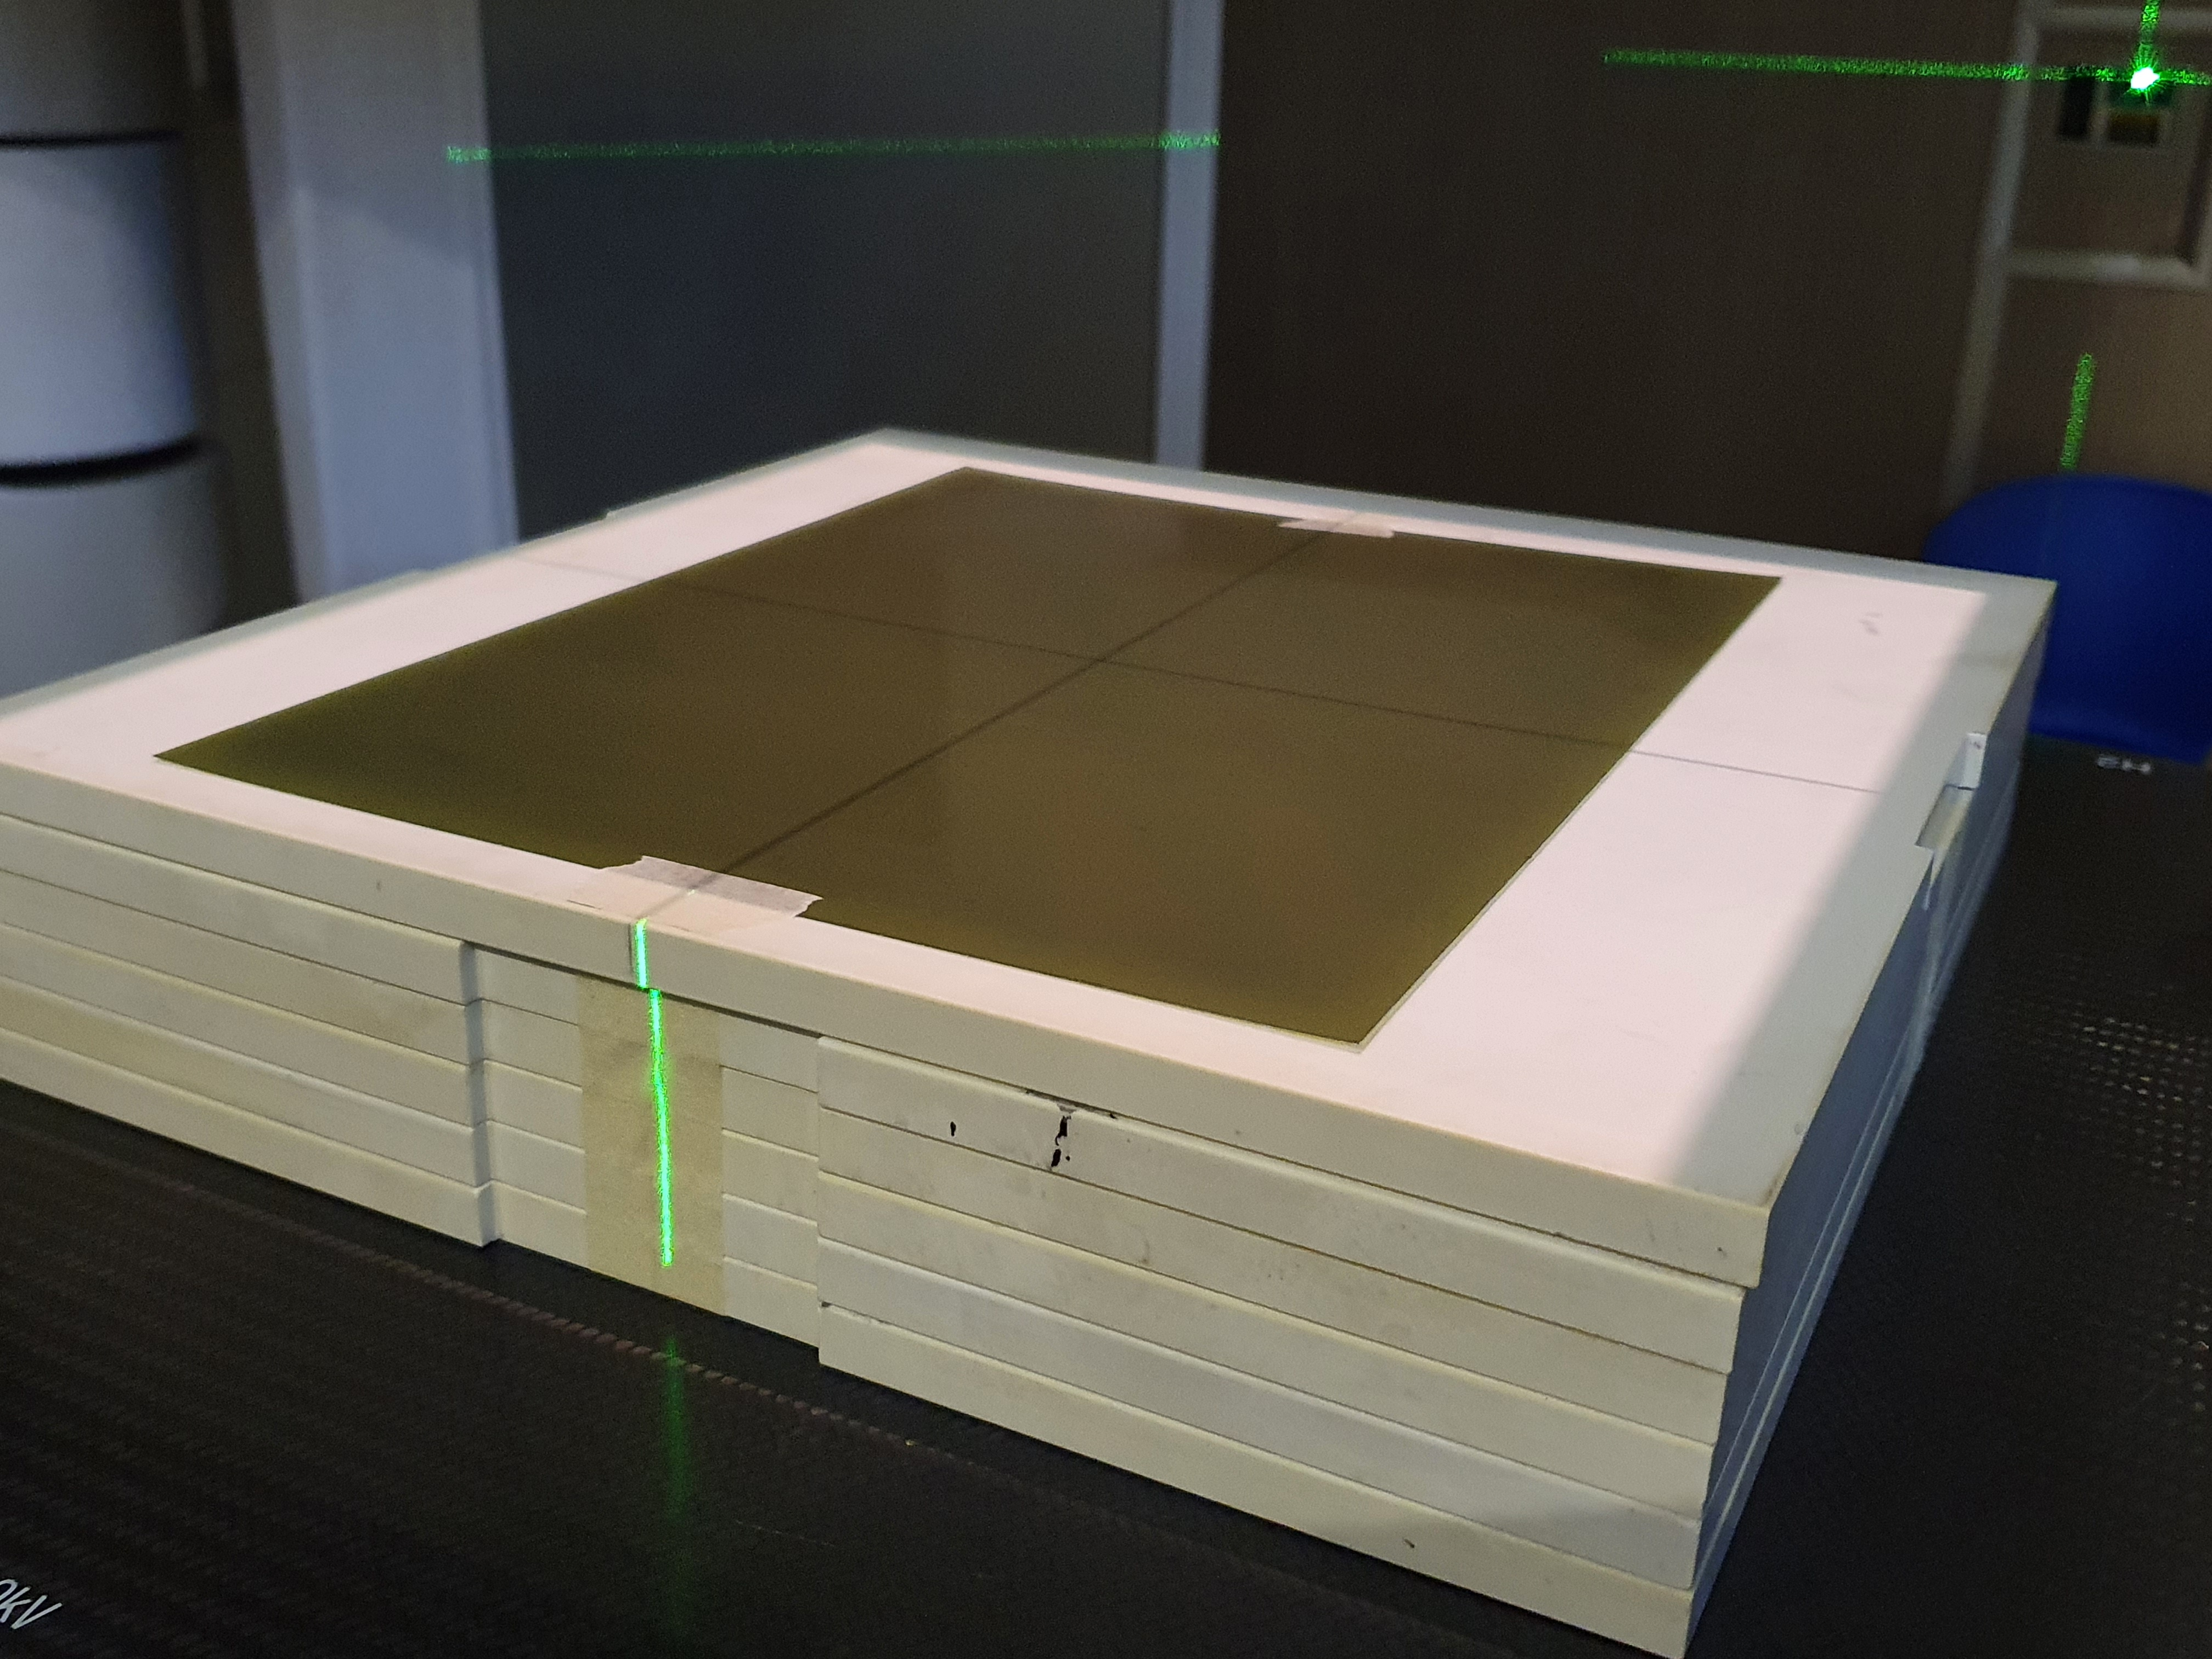
\includegraphics[width=0.7\linewidth]{images/alineacionCampo.jpg}
	\caption{Alineación de la película ajustada con el isocentro del acelerador}
	\label{fig:MontajePelicula}
\end{figure}

Con el objetivo de medir los cambios de coloración que se dan debido a la radiación, se planeó irradiar películas con dosis entre 0 y 20 Gy. Con el objetivo de comprobar que el cambio de color fuera unívocamente correspondiente a la dosis depositada, por cada dosis elegida se irradiaron tres películas, para luego comparar su cambio de coloración y determinar si se reproduce el mismo cambio en las tres.\\ 


Para determinar experimentalmente las dosis que se irradiaron se usó un montaje con una cámara de ionización Farmer 30010 PTW Freiburg GmbH junto con un electrómetro, siguiendo el protocolo TRS398 descrito anteriormente. Así, por cada cantidad fija de unidades monitor que se programaron con la máquina, se realizó la medición de la dosis efectiva depositada a la misma profundidad de agua solida y distancia a la fuente que se usó en la irradiación de las películas. Esta medición se realizo diez veces para las primeras cuatro dosis, siete veces para la quinta dosis, cinco veces para las siguientes tres y finalmente tres veces para las últimas tres dosis. El montaje de lectura con el electrómetro se muestra en la figura \ref{fig:Montajeelectrometro}\\
\begin{figure}[H]
	\centering
	% \missingfigure is from todonotes
	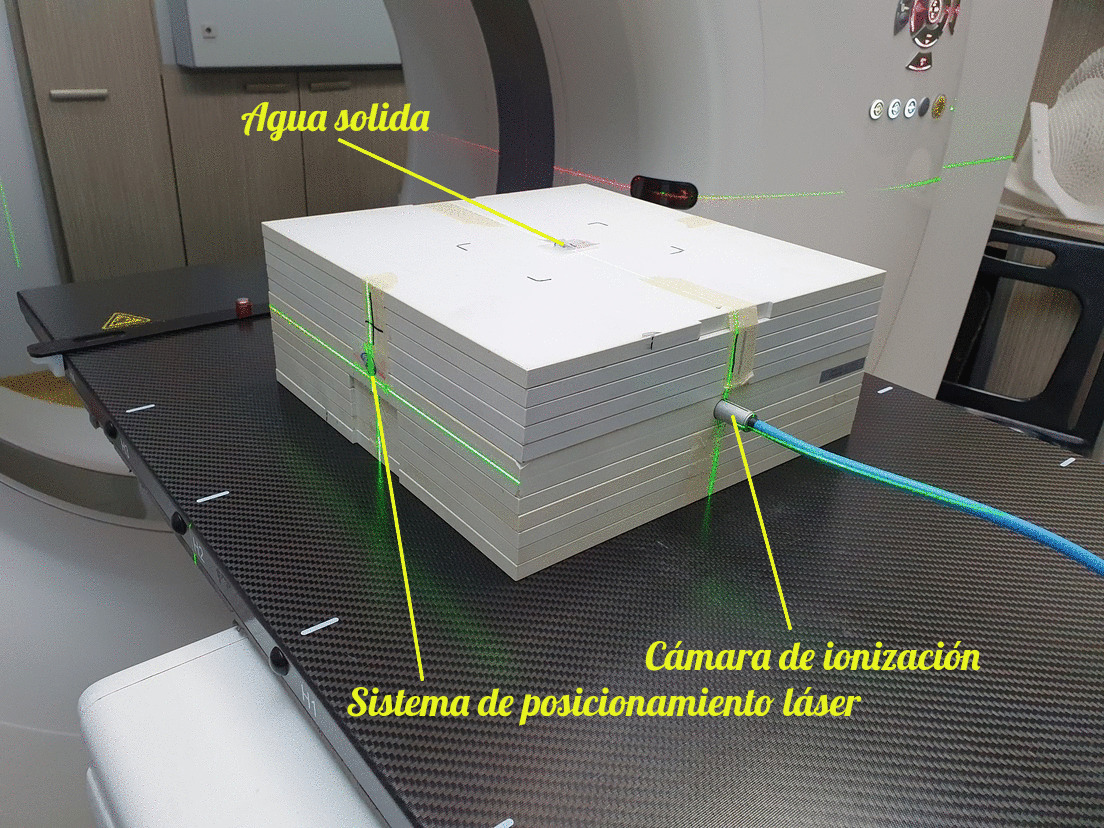
\includegraphics[width=0.7\linewidth]{images/elctrometro.jpg}
	
	\caption{Montaje para determinación de dosis}
	\label{fig:Montajeelectrometro}
\end{figure}

La cantidad de unidades monitor que se requieren entregar para lograr determinada dosis absorbida en el plano de la película se calcularon mediante el sistema de planeación Eclipse. Para esto se tomó un TAC del agua solida y la cámara de ionización y se reconstruyó la geometría bajo la cual fueron realizados los cálculos.\\

Por otro lado, para realizar comparaciones entre mapas de dosis de tratamientos calculados con el sistema de planeación y los mapas de dosis obtenidos mediante la calibración  se irradiaron dos planes. En primer lugar, se irradió un plan pirámide, que en el plano de la película produce un mapa de dosis calculado por el sistema como se ilustra en la figura \ref{fig:TPSPiramide}\\

\begin{figure}
	\centering
	% \missingfigure is from todonotes
	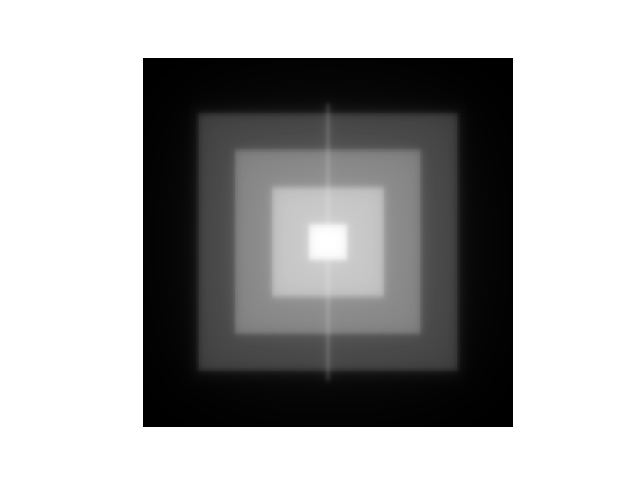
\includegraphics[width=0.7\linewidth]{images/piramideTPS.png}
	\caption{Mapa de dosis calculado por el sistema de planeación en el plano de la película para el plan pirámide}
	\label{fig:TPSPiramide}
\end{figure}

Posteriormente, se irradió un plan de tratamiento IMRT de cáncer de mama colapsado a 0°, es decir, todos los campos del plan fueron irradiados de forma perpendicular a la película. Este plan produjo un mapa de dosis en el plano de la película calculado por el sistema de planeación que se ilustra en la figura \ref{fig:TPSMama}\\

\begin{figure}
	\centering
	% \missingfigure is from todonotes
	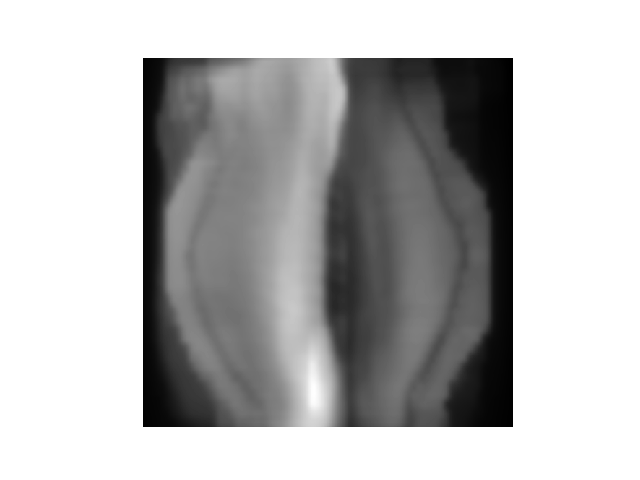
\includegraphics[width=0.7\linewidth]{images/mamaTPS.png}
	\caption{Mapa de dosis calculado por el sistema de planeación en el plano de la película para el plan de tratamiento de mama}
	\label{fig:TPSMama}
\end{figure}

Por otro lado, también se irradio un cuadrado con 5 Gy usando las láminas del MLC para formar un campo de 10 x 10 cm para realizar la comprobación más sencilla de la eficiencia del proceso de calibración.\\

Finalmente, se calcularon los mapas de dosis obtenidos mediante las películas y se compararon con los mapas calculados usando diversas herramientas, incluyendo el análisis $\Gamma$.

\section{Escaneo y tratamiento}
Para la fase de digitalización se usó un escáner ScanMaker 1000XL en modo de transmisión que tiene un área operativa de 30.48 cm x 40.64 cm, eligiendo el modo RGB con 16 bits por canal, desactivando los filtros y correcciones automáticas y usando una resolución de 100 ppi siguiendo las recomendaciones propuestas en \cite{Devic2016}. Con esta configuración, se obtienen imágenes a color en formato TIFF de alrededor de 10 MB de tamaño, dependiendo del tamaño del área escaneada. Esta imagen sin ningún tipo de compresión se puede traducir a una matriz de pixeles con valores entre $0$ y $2^{16}-1$ por cada canal de color que puede ser leída mediante diferentes paquetes de programación. En este caso se usa la librería de python tiffread para la lectura. \\



En la figura \ref{fig:fondoNegro} se muestra una imagen del escáner cuando la lampara fue opacada con abundante cartulina negra. Para corregir estos pixeles se usó una combinación entre las técnicas de supresión de ruido con background y filtrado con filtros de Wiener y mediana. \\

Para reducir efectos de dependencia de posición, se usó siempre la parte central superior del escáner para digitalizar las imágenes. De esta manera, el sesgo sería siempre el mismo y podría ser corregido con el método multicanal propuesto.\\

En \cite{Micke2011} se reporta que este método para predecir dosis aporta en la separación de cambios de color debidos a defectos del escáner y cambios de color debidos a la irradiación propiamente. En la figura \ref{fig:Multicanal} se evidencia como el uso de este método puede usarse para separar la parte dependiente de la dosis del color de la parte que es dependiente de las heterogeneidades del escáner, en este caso se usa el ejemplo propuesto en \cite{Micke2011}. \\

\begin{figure}
	\centering
	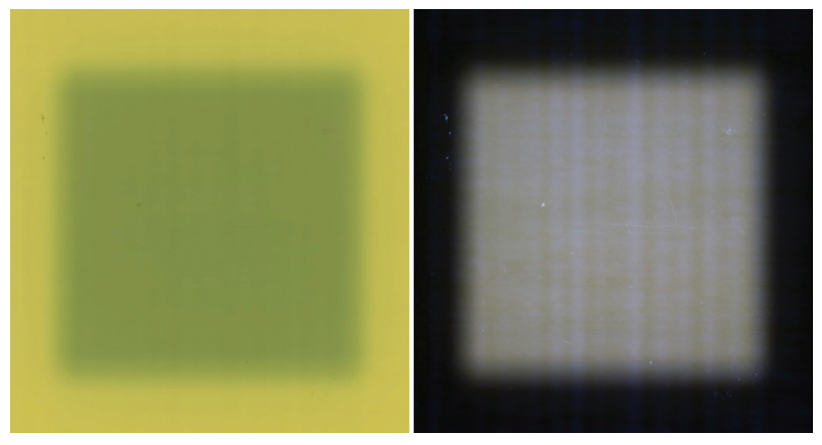
\includegraphics[width=0.7\linewidth]{images/imagenMicke.png}
	
	\caption{Separación de parte dependiente de dosis\cite{Micke2011}}
	\label{fig:Multicanal}
\end{figure}

Además, para corregir este efecto de mejor manera, el programa también incluye la opción de restar el sesgo a cada medida a partir de una medida de una película sin irradiar. De esta manera, el cambio de coloración es ajustado con respecto a como varía la respuesta en función de la ubicación escaneada. \\

De la misma manera, se implementó el uso de filtros para corregir particularidades del escáner como pixeles dañados y rayones en la película o escáner. El filtro recomendado en la literatura para estas circunstancias es el filtro de Wiener \cite{Devic2016}, el cual se implementó en el programa. \\

También es posible usar el filtro en el cual el valor de transmitancia en cada pixel se remplaza con el promedio de los valores que lo rodean, eliminando parcialmente ciertas inhomogeneidades que podrían presentarse. Otro filtro posible es el filtro de mediana, que reemplaza en cada pixel su valor por el que más se repite a su alrededor en cierto intervalo. \\

La eficiencia de estos filtros es dependiente de la calidad de la imagen obtenida, por lo que para cada digitalización se probaron diferentes combinaciones de estos, siendo los más eficientes, en la mayoría de los casos, el filtro de la mediana y el filtro de Wiener.\\

Aunque la aplicación de filtros ayuda de cierta manera a reducir los efectos de las heterogeneidades de fabricación, estos no lo solucionan por completo, puesto que estas son de carácter no local. La mejor manera de incrementar la seguridad con respecto a este tipo de incertidumbre es realizando varias irradiaciones en  diferentes películas y comparando sus resultados.\\


Por otro lado, el fabricante del lote de películas EBT3 usado reporta que en el último control de calidad realizado, las películas presentaban una homogeneidad superior al 95 \% sobre su superficie, es decir, la estructura física de la película podía variar 5\% en sus dimensiones en algunas secciones. Esto no implica directamente una desviación de más de 5\% en el color medido por esta inhomogeneidad, puesto que la capa activa permanece generalmente uniforme, pero si afecta de cierta manera relativamente sutil la medida. Este efecto también puede ser corregido mediante el método multicanal. \\ 



Finalmente, para evitar cambios en la medida por efectos de la orientación de la película en el escáner, se escaneó siempre usando la orientación horizontal en la parte superior del escaner.\\








